%!TEX root = ../thesis.tex
%*******************************************************************************
%*********************************** First Chapter *****************************
%*******************************************************************************

\chapter{Introduction}  %Title of the First Chapter


% **************************** Define Graphics Path **************************
%\ifpdf
%    \graphicspath{{chapter1/figs/raster/}{chapter1/figs/PDF/}{chapter1/figs/}}
%\else
%    \graphicspath{{chapter1/figs/vector/}{chapter1/figs/}}
%\fi
\graphicspath{{figs/chapter1/PDF/}}

%%**************************** %Broad Purpose  **********************************
%* How long (number of words)?
%* Deadline
%* What have you got?
%


%%********************************** %First Section  **************************************
\section{Background}
Human movement is a complex system where not only multiple
joints and limbs are involved for a specific task in a determined environment
but also how we process the external information with all of our available senses 
and use our experiences, which play a crucial role in the way each person moves.
Recent studies in human motion recognition have revealed the possibility to estimate
features from lower dimensions signals to distinguish differences between 
styles of pedalling motion \cite{Quintana-Duque2012, Quintana-Duque2016}, 
to perform gait identification \cite{sama2013, frank2010} 
or to do pattern recognition from biological signals \cite{gomezgarcia2014}.

The lower dimension signals from biological signals are generally time series 
of $1-$dimension in $\mathbb{R}$ which commonly have 
high nonlinearity, complexity, and non-stationarity \cite{gomezgarcia2014},
where traditional methods in time-domain or frequency-domain 
tend to fail to detect tiny modulations in frequency or phase \cite{marwan2011}.
However, methods of nonlinear time series analysis can objectively quantify such 
human movement variability \cite{Quintana-Duque2012, Quintana-Duque2016, sama2013, 
frank2010, gomezgarcia2014, marwan2011, stergiou2011, packard1980}.
With this in mind, \cite{bradley2015} reviewed methods for
nonlinear time series analysis which provide the foundationsto reconstruct the state space methodology (RSS) \cite{takens1981},
recurrence plots (RP) \cite{eckmann1987}, 
recurrence quantification analysis (RQA) \cite{zbilut1992} and others.
Such methodologies are implemented very easily using embedding paramters ($m$ and $\tau$).
However, the computation of embedding parameter is still an open problem
since there is no general technique to compute the embedding parameters 
becuase time series are system-dependent meaning that these may only work 
for one purpose (e.g., prediction) and may not work well for another purpose
(e.g., computing dynamical invariants) \cite{bradley2015}.


In addition, the quality of the time series is important to have 
reliable results. For instance, methodologies to compute embedding parameters 
e.g., autocorrelation, mutual information, and nearest neighbour 
require data which is well sampled and with little noise \cite{garland2016} 
or need purely deterministic signals \cite{kantz2003}.
Similarly, methodologies such as RSS, RP and RQA can break down with real-world 
datasets which have generally different length, 
different values of accuracy and precision \cite{frank2010},
%(rounding errors due to finite precision of the measurement apparatus which include frequency acquisition \cite{frank2010}),
and data may be contaminated with different or unknown sources of noise \cite{garland2016}.
It is surprising that even with the previous constraints with regard to 
the quality of data, and the problem with the estimation of embedding parameters,
the results of analysis using nonlinear dynamics 
have proven to be helpful to understand and characterise time series 
\cite{Quintana-Duque2012, Quintana-Duque2016, sama2013, frank2010,
gomezgarcia2014, marwan2011, stergiou2011, bradley2015}.
Another point to consider with time series analysis using nonlinear dynamics
is the appropriate use of post-processing techniques such as 
interpolation, filtering or normalisation.
It can then be said that there is little research and understanding 
on the effects for post-processing techniques in the interpretation of RSSs, RPs 
and metrics of RQA.

%Also \cite{bradley2015} reviewed the use of Recurrence Plots (RP) and 
%Recurrence Quantification Analysis (RQA), both of which show the recurrences of a given $n$-dimensional system  
%in a two-dimensional map of black/white dots, which help 
%to have a more intuitive meaning of the time series.
%Probably, the most important results of \cite{iwanski1998} is that 
%RQA are quantitatively and qualitatively independent of embedding 
%dimension which was also experimentally verified.
%However, the estimation of embedding parameters and finding the right
%parameters to perform RQA is still an open problem.
%









\section{Research questions and contributions}

A number of questions regarding movement variability has been investigated
\cite{stergiou2006, stergiou2011}.
"How is variability controlling while learning a new skill?" \cite{wagner2012, seifert2011, bartlett2007}, 
"Is variability associated with disease/health?" \cite{stergiou2006, stergiou2011},
"What are the sources of variability and how do they interact in the production
of observed variation of movement?" \cite{preatoni2007, preatoni2010, preatoni2013}.
However, little has been investigated about the realiability of 
nonlinear tools to quantify movement variability \cite{iwanski1998, yao2017}
Therefore, for this thesis, it is explored the effects on RSSs, RPs and metrics of RQA
with different features of time series such as structure, 
levels of smoothness and window lengths.
To do such exploration, an experiment is conducted with twenty 
right-handed healthy participants in the context of 
human-humanoid imitation activities where participants 
were asked to imitate simple arm movements performed 
by a humanoid robot. Participants and humanoid robot worn 
inertial sensors that collected time series.
Hence, the following research questions are investigated:


\begin{itemize}

\item What are the effects on RSSs, RPs, and RQA metrics
	for different embedding parameters, different recurrence thresholds 
	and different characteristics of time series (window length, smoothness of the signal, structure)?

\item How much smoothing of the raw signal is appropriate in order to capture the
	nature of the variability?

\item How sensitive or robust are RQA metrics to quantify movement variability?

\end{itemize}






\section{Structure of this thesis}

This thesis is organised as follow. 
Section 2 presents a review of the state space reconstruction 
that includes an explanation for uniform time delay embedding and a 
description of the techniques to estimate of minimum embedding 
parameters (e.g. false nearest neighbour and average mutual information).
Section 3 presents an introduction to Recurrence Plots,
structures of Recurrence Plots and different metrics to perform Recurrence Quantification Analysis.
In section 4, an experiment in the context of human-robot imitation
activities is presented where description of participants, data collection from inertial measurement unit sensors,
and preprocessing techniques (e.g raw data, normalised data, smoothed data and windowing)
are given.
In section 5, results for RSS, RP and RQA are presented understand 
movement variability both between participants and activities, 
as well as the variation of smoothness of the time series.
The research is finalised in conclusion and future work.



%---------------------------------(FIGURE)-------------------------------------
\begin{figure}
\centering
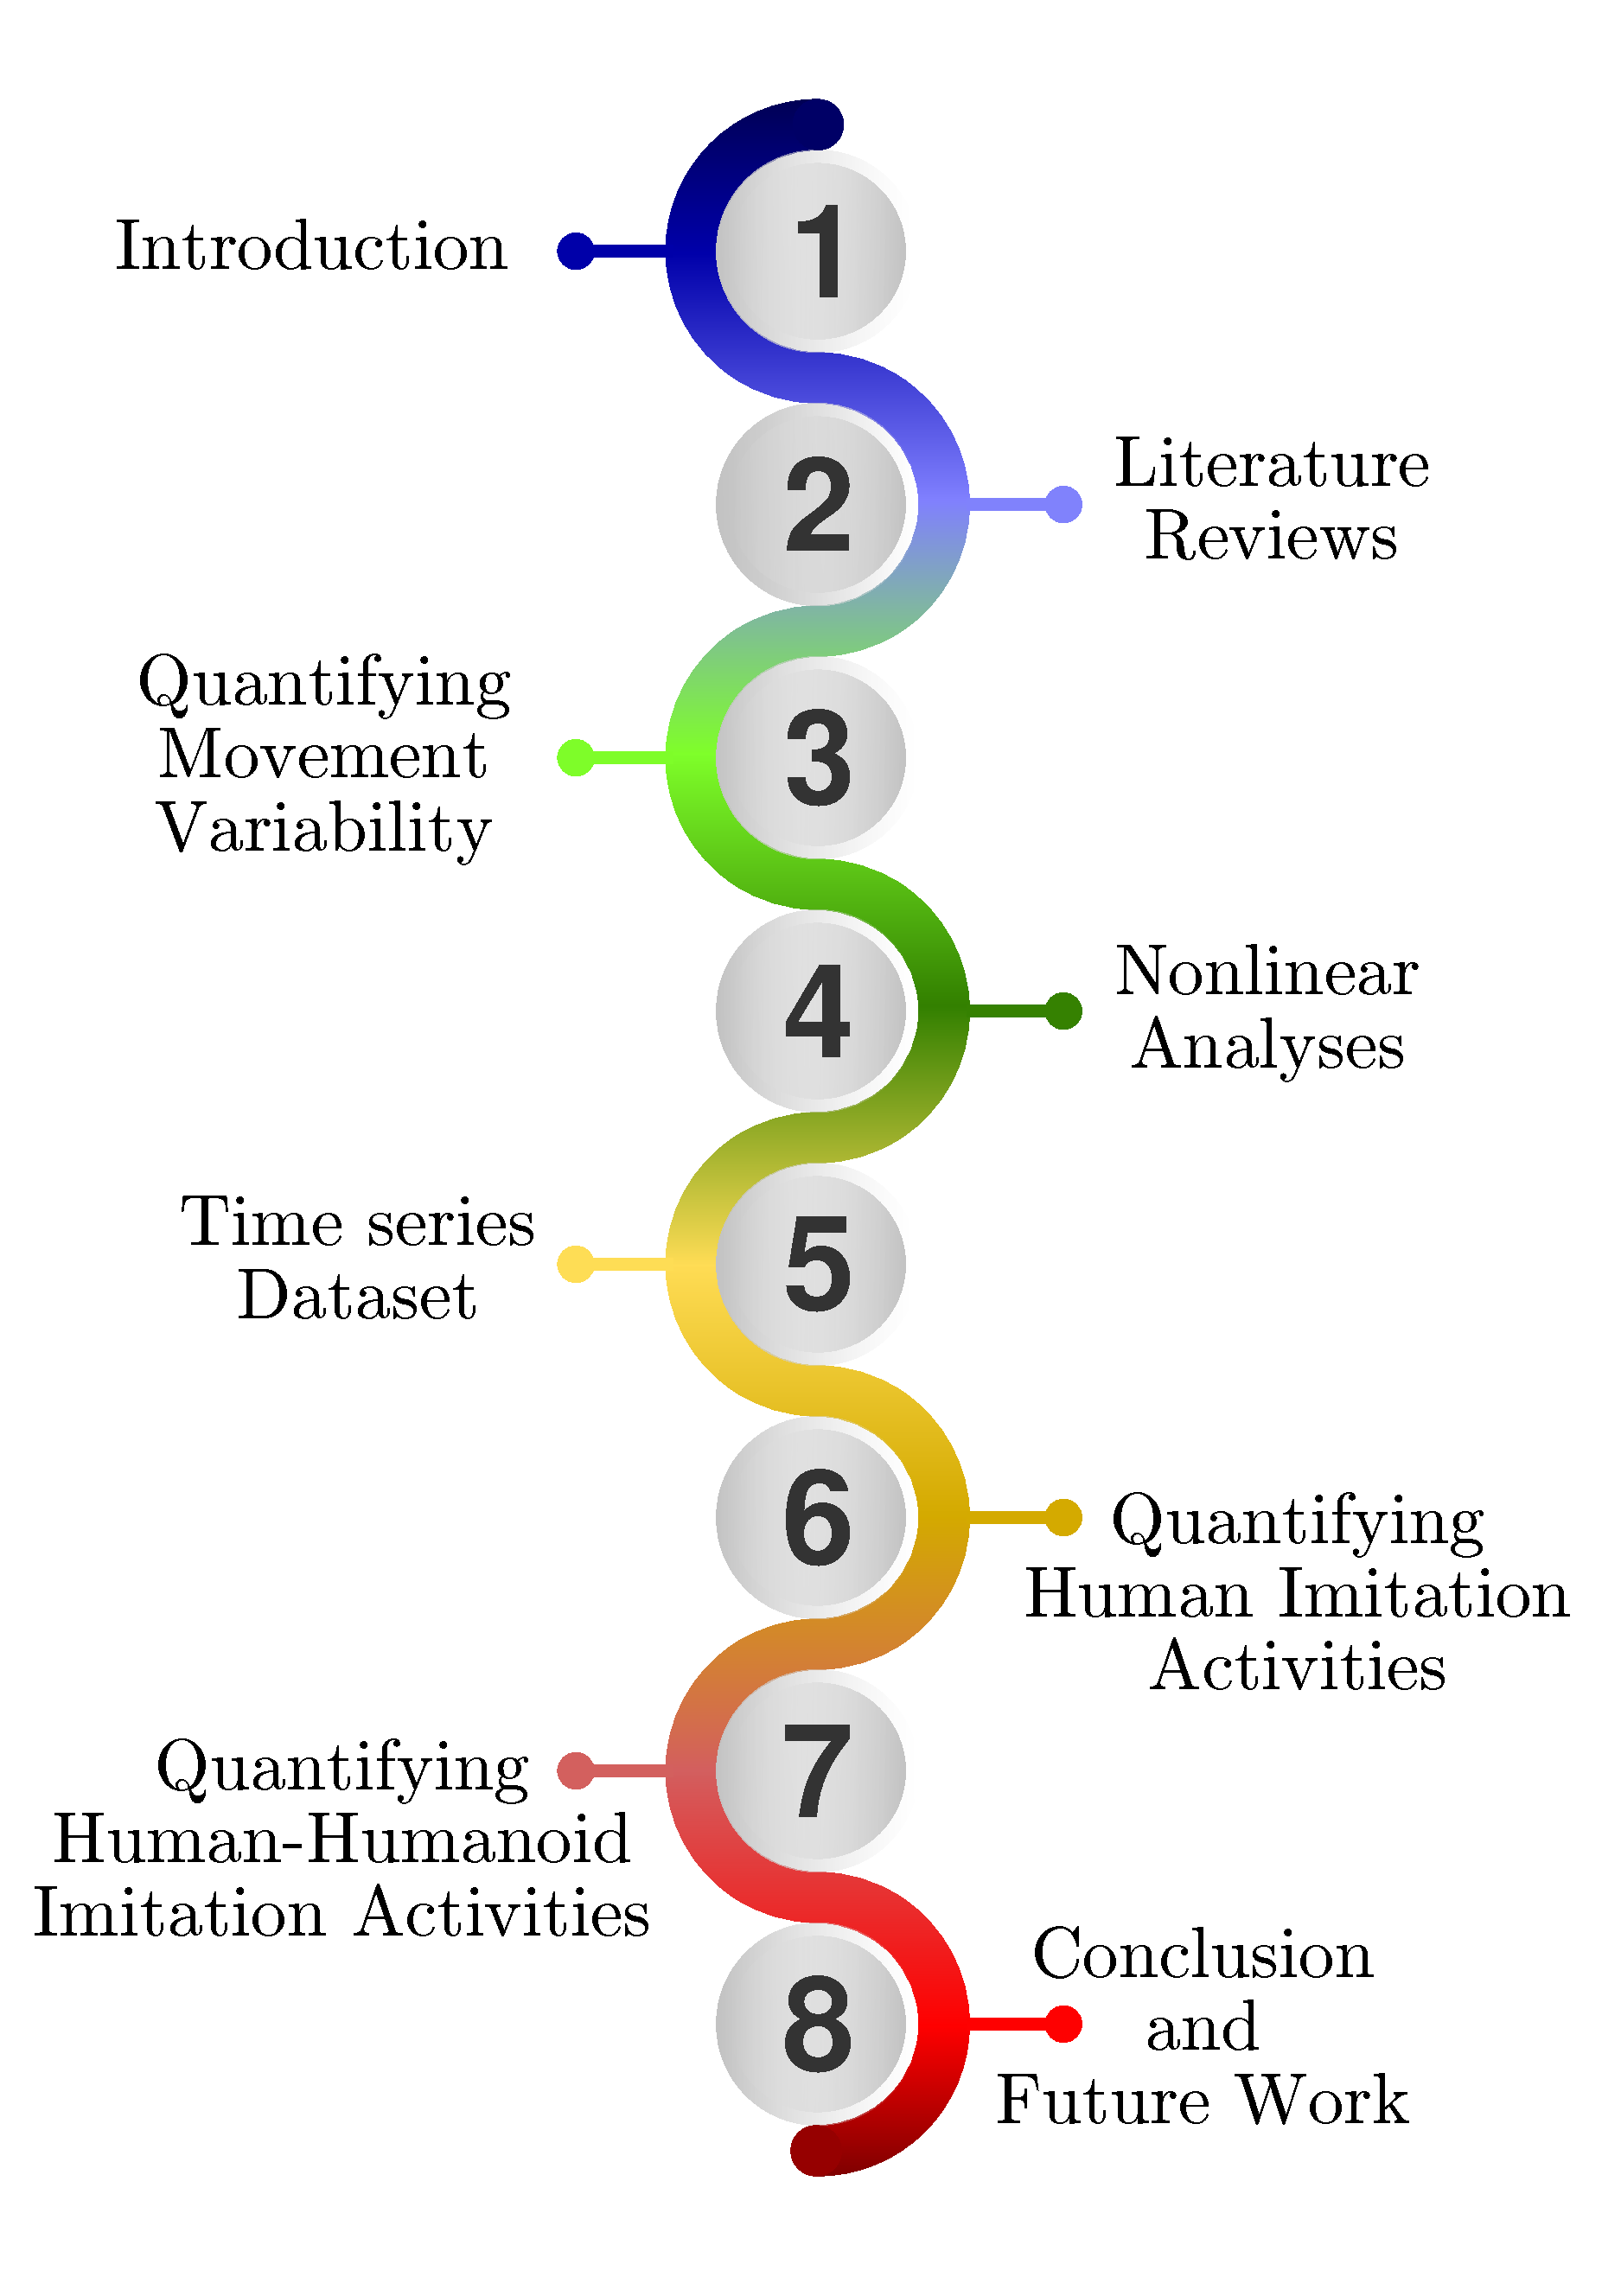
\includegraphics[width=1.0\textwidth]{thesis-structure-v02}
    \caption{
	{\bf Thesis structure.}
	One to eight numbers represent the chapter number.   
	  }
    \label{fig:ts}
\end{figure}
%%---------------------------------(FIGURE)-------------------------------------





\section{Publications}
Partial work of this thesis has been published in the following peer-reviewed conferences.
\begin{itemize}
\item Xochicale M., Baber C., and Oussalah M.,
	Understanding Movement Variability of Simplistic Gestures Using an Inertial Sensor,
	in Proceedings of the 5th ACM International Symposium on Pervasive Displays, 
	Oulu, Finland, June 2016, 
	pages 239--240.

\item Xochicale M., Baber C., and Oussalah M.,
	Analysis of the Movement Variability in Dance Activities Using Wearable Sensors,
	in Wearable Robotics: Challenges and Trends,
	Segovia, Spain, October 2016,
	pages 149--154.

\item Xochicale M., Baber C., and Oussalah M.,
	Towards the Quantification of Human-Robot Imitation Using Wearable Inertial Sensors,
	in Proceedings of the Companion of the 2017 ACM/IEEE International Conference on Human-Robot Interaction,
	Vienna, Austria, March 2017,
	pages 327--328.

\item Xochicale M., and Baber C.,
	Towards the Analysis of Movement Variability in Human-Humanoid Imitation Activities,
	in Proceedings of the 5th International Conference on Human Agent Interaction,
	Bielefeld, Germany, October 2017,
	pages 371--374.
\end{itemize}


